\chapter{Implementierungs}

\section{Build System}
Der Build Prozess ist ein Prozess, welcher alle Schritte beinhaltet um aus dem vorhandenen Source Code eine ausführbare Software zu erstellen. Insbesondere werden dabei benötigte Abhängigkeiten zur Verfügung gestellt und in die Software integriert, der Source Code kompiliert und alle Software Teile in einem ausführbaren Format zusammengeführt. Dieser Prozess kann sehr komplex werden und ist daher häufig fehleranfällig. Unter anderem die Kombination von mehreren Build Systemen und unterschiedlichen Programmierumgebungen wird dabei als ein Kernproblem angesehen\cite{buildSystemProblem}. Da sich dieses Projekt in ein Frontend und Backend mit unterschiedlichen Programmiersprachen gliedert, ist es allerdings notwendig unterschiedliche Build Systeme zu integrieren. Dies ist erforderlich, da die existierenden Systeme sich eher auf eine Umgebung spezialisieren und zum Beispiel nur Abhängigkeiten einer Programmiersprache in einem zentralen Repository anbieten (z.B. npm registry für JavaScript oder maven central für Java Anwendungen). Auch existieren bestimmte Plugins, zum Beispiel für das Transpilieren von TypeScript, nicht für alle Build Systeme. Alles in allem erhöht sich zwar die Build Komplexität und Dauer, allerdings hat es auch Vorteile. Zum einen führt es dazu, dass das Frontend vom Backend vollständig isoliert ist und die reine Frontendentwicklung ohne unnötige Abhängigkeiten und Build Prozesse ablaufen kann. Zum anderen erweitert sich dadurch auch die Auswahl an vorhanden Tools und Plugins, was die Entwicklung deutlich vereinfachen kann.

Für dieses Projekt wird Maven als System für das Backend und npm als System für das Frontend genutzt. Die Entscheidung wurde auf Grund der hohen Beliebtheit und der persönlichen Expertise mit diesen Tools getroffen. Aus reiner Systemsicht ist das Frontend ein Teil des Backends, da es für die Auslieferung des Frontends an den Nutzer verantwortlich ist. Der Build beginnt daher auch in Maven. Als erstes muss sichergestellt werden, dass npm und Node.js auf dem Rechner vorhanden sind. Für die Kommunikation mit diesen wird das frontend-maven-plugin\footnote{\url{https://github.com/eirslett/frontend-maven-plugin}} genutzt, welches sie in einem ersten Schritt in einen lokalen Ordner installiert, solange sie noch nicht vorhanden sind. Anschließend wird “npm install” aufgerufen, um alle deklarierten Abhängigkeiten aus dem Frontend zu installieren. Dazu zählt zum Beispiel Three.js oder auch der TypeScript Transpiler. Anschließend wird der Build an das Frontend übergeben, indem ein fest definiertes npm Script aufgerufen wird. Dieses führt als erstes den TypeScript Transpiler aus um die benötigten JavaScript Dateien anzulegen. Da npm eigentlich ein Build-Tool für Node.js, welches lokal in einem Server ausgeführt wird, müssen die Abhängigkeiten für die Verwendung im Browser besonders behandelt werden. Hier ist ein sogenannter Bundler erforderlich, welche alle Abhängigkeiten in einer lokalen Datei zusammenfasst, welche dann an den User ausgeliefert wird. Als erstes wurde das Tool Browserify in Betracht gezogen, was ein existierendes NodeJS-Projekt ohne Codeänderungen für den Browser vorbereitet. Es wurde sich jedoch für das Tool Webpack entschieden, hauptsächlich auf Grund des direkten Supports von JavaScript Modulen ohne weitere Abhängigkeiten. Die Nutzung eines Bundlers hat des Weiteren des Vorteil, dass der Code minifiziert wird und in einer einzigen Datei zusammengefasst wird, was ein deutlich schnelleres Laden der Webseite zur Folge hat. Im Gegenzug verliert man die Fähigkeit, den Frontend Code zu debuggen, da die Minifizierung dabei natürlich stark stört. Dies kann allerdings durch die Verwendung von Source Maps verhindert werden, die für genau diesen Zweck eine Zuweisung von minifizierten zu originalen Variablen- und Methodennamen zur Verfügung stellen. Um das Frontend jetzt per Webserver an den User auszuliefern, müssen die Dateien jetzt in einen Ordner im Java Classpath befördert werden. Wichtig dabei ist, dass nur die benötigten Dateien verschoben werden dürfen, da diese sonst über den Webserver erreichbar wären. Dies wäre insbesondere bei den diversen Konfigurationsdateien ein Sicherheitsproblem. Auch das Verschieben des node\_modules Ordner wäre ein grober Fehler, da dies zu einer relativ großen ausführbaren Datei führen würde. Anschließend geht der Build im Backend mit dem Kompilieren der Java Dateien weiter. Nachdem alle Tests automatisch durchlaufen wurden, werden dann alle Abhängigkeiten des Backends, unter anderem der Undertow Server, zu einem fertigen Artefakt (Fat JAR) zusammengeführt, welches dann auf einen Server deployed und dort ausgeführt werden kann.

\section{Visualisierung}
Für die eigentliche Visualisierung kommen Shader zum Einsatz. Dafür muss dem Shader natürlich der Höhenwert bekannt sein. Bei einer flachen Projektion lässt sich dieser aus dem Vertex ablesen (entsprechend skalierte y-Koordinate), dies ändert sich natürlich, sobald eine sphärische Projektion zum Einsatz kommt. Die einfachste Möglichkeit ist es, dem Shader den Höhenwert in Metern neben dem Vertex als weiteres Attribut zu übergeben. Da dies die theoretische maximale Speichernutzung allerdings um weitere 4 GB erhöhen würde, was einer Erhöhung um 1/3 der Gesamtmenge entspricht, wurde dieser Ansatz verworfen. Stattdessen ist effizienter, den Höhenwert aus dem Vertex zu berechnen. Da der Höhenwert immer der Abweichung von einem vordefinierten Radius entspricht (ähnlich dem "Meeresspiegel" auf der Erde), muss dieser Radius einfach von der Länge des Vertex abgezogen werden. Dies funktioniert allerdings nur, wenn der Mittelpunkt des Modells auch mit dem Koordinaten-Nullpunkt übereinstimmt, da nur dann die Länge des Vertex der Distanz zum Punkt auf der Oberfläche entspricht. Um dies im Vertexshader zu implementieren, müssen ihm die verwendete Projektion, der Radius und die Skalierung von GL Einheiten zu Metern bekannt sein. Diese werden als Uniform Werte übergeben, sind also nicht abhängig von der Vertex-Anzahl und spielen daher für die maximale Speichernutzung keine Rolle. Der Vertexshader berechnet also wie beschrieben die Höhe in Metern und gibt sie an den Fragmentshader weiter. Des Weiteren transformiert er wie üblich den Vertex mit der Model-Matrix (enthält die Transformationen des Modells), der View-Matrix (enthält die inversen Transformationen der Kamera) und der Projektions-Matrix (enthält die perspektivische Transformation der Kamera) um die endgültige Position des Vertex zu bestimmen.

Der Fragmentshader hat nun die Aufgabe, aus diesem Höhenwert einen Farbwert zu generieren. Eine Möglichkeit wäre es, einfach verschiedene Grenzen zu definieren und diesen Grenzen feste Farbwerte zuzuweisen. Dann kann geprüft werden, welchem Bereich der Höhenwert entspricht und der endgültige Farbwert entspricht dann einer Variation des Farbwerts des Bereichs. Da dies allerdings mehrere Verzweigungen (conditionals) zur Prüfung der Grenzen erfordert und dies in der Shaderentwicklung vermieden werden sollte\footnote{siehe \cite{shaderDev}, Kapitel 14, Abschnitt Avoid Dynamic Branching, S. 273}, wurde eine bessere Lösung gesucht. Insbesondere, da es sich um das sogenannte dynamic branching handelt, da da die Bedingung abhängig vom Höhenwert ist, welcher natürlich pro Vertex anders ist. Des Weiteren wurde auf Grund der Datenmenge die kritischste Stelle der Performance (bottleneck) eher auf GPU Seite angesehen, sodass hier dringender auf der Performance geachtet werden sollte. Schlussendlich wurde der Fakt genutzt, das der Hue-Wert im HSV-Farbraum eine relativ lineare Verteilung verschiedener Farben enthält und so gut als Farbskala genutzt werden kann. Da die Ausgabe des Shaders allerdings im RGBA-Format erfolgen muss, ist hier eine Umwandlung des HSV Werten in diesen Farbraum erforderlich. Es wird also der Prozentwert des aktuellen Höhenwerts abhängig von vom Nutzer definierten Grenzen berechnet und diesem Prozentwert ein Hue Wert zugeordnet. Dabei wurde der Farbraum vorher noch verkleinert und invertiert, sodass die Farben dann von einem Blau-Ton (niedrigster Wert) zu einem Rot-Ton (höchster Wert) reichen. 

\section{Kamerabewegung}
Die erste Implementierung war eine frei im Raum bewegbare Kamera, welche man mit der Tastatur steuern konnte. Als konkrete Tasten wurden zum einen die Pfeiltasten als auch die übliche Alternative WASD genutzt. Diese sind allgemein als Steuerungstasten bekannt und sollten daher keiner Erklärung bedürfen. Die Kamera bewegte sich dabei entlang des lokalen Koordinatensystems der Kamera. Dieses kann dann mit der Maus entlang der x-Achse (pitch) und y-Achse (yaw) gedreht werden. Eine Drehung um die z-Achse (roll) verkompliziert die Steuerung und wurde daher bewusst nicht implementiert. Eine Bewegung der Maus auf der x-Achse führt dabei zu einer Rotation der Kamera entlang der y-Achse und eine Bewegung auf der y-Achse zu einer Rotation entlang der x-Achse. Die Blickrichtung der Kamera folgt also effektiv der Bewegung der Maus. Dabei wurde das Drehen nur beim Gedrückthalten der Maustaste (dragging) durchgeführt, da die Kamera sich sonst natürlich bei der normalen Navigation auf der Seite bewegen würde. Das Gedrückthalten ist dabei schon weniger intuitiv, allerdings entspricht es der physischen Bewegung des Ziehens an einer Seite des Globus in der realen Welt. Hier ist allerdings eine genauere Evaluation der Steuerung notwendig um eine gute User-Experience zu gewährleisten.

Wichtig bei der Implementierung ist, dass die Geschwindigkeit der Bewegung nicht von der Geschwindigkeit des Browser abhängen darf. Daher müssen alle Vektoren, welche eine Bewegung darstellen, mit der Zeit multipliziert werden, die seit dem letzten Aufruf der Bewegung vergangen ist. Nur so wird in einem bestimmten Zeitabschnitt immer die gleiche Länge zurückgelegt. Ein weiterer Aspekt ist, dass das Gedrückthalten einer Taste natürlich zu einer kontinuierlichen Bewegung führen soll. Um dies zu erkennen kann zum einen das keydown-Event des Browser genutzt werden, welches auch gesendet wird, solange die Taste gedrückt bleibt. Allerdings ist dabei eine spürbare Verzögerung zwischen erstem und nachfolgenden Events vorhanden, sodass die Bewegung initial ziemlich ruckartig erfolgt. Auch ist die Geschwindigkeit, mit der die Events gesendet werden, nicht definiert und kann so zu sehr ruckartigen Bewegungen führen, sollte die Rate weit unter der Bildwiederholrate des Monitors liegen. Stattdessen werden die Kameras in der Render-Schleife, begrenzt durch die Bildwiederholungsrate (vSync), so lange in der gleichen Konfiguration geupdated, bis ein entsprechendes keyup-Event der gleichen Taste registriert wurde.

Die zweite Implementierung ist die stationäre Kamera, welche sich um den Globus in einem festen Abstand bewegt. Auch hier wurde die Rotation durch das Dragging der Maus implementiert. Da beide Kameras die selben Steuerungsmöglichkeiten besitzen sollte dies für den User schnell verständlich sein. Der Abstand zum Globus kann dabei mit dem Mausrad verändert werden, was auch sehr intuitiv sein sollte. Beim ersten Ansatz der Implementierung wurde die Kamera zum Rotierungspunkt (Pivot) bewegt, um den entsprechenden Winkel rotiert und anschließend im lokalen Koordinatensystem entlang des ursprünglichen Bewegungsvektors zurück bewegt. Ein wesentlich einfacher und genauerer Ansatz wurde dann in der Form des Scene-Graphs der THREE Bibliothek gefunden. Dabei wird eine Hierarchie an Objekten in Form einer Baumstruktur definiert und alle Transformationen eines Objektes werden automatisch an dessen Kinder weitergegeben. Wenn jetzt die Kamera als Kind des Pivot definiert wird, dann kann dieser normal rotiert werden und die Kamera rotiert automatisch im selben Winkel und Abstand mit. Für das Zoomen wurde das wheel-Event genutzt, welches Informationen darüber enthält, wie stark das Mausrad rotiert wurde. Hier gibt es die unterschiedlichen Einheiten Pixel, Zeilen und Seiten, welche auf die Navigation einer normaleren Seite mit Text ausgelegt sind. In konkreten Fall wurde nur die Scrollrichtung ermittelt und die Kamera mit einem festen Betrag entlang der lokalen z-Achse verschoben. Zusätzlich wurden minimale und maximale Abstände definiert und von der Implementation beachtet, damit die Kamera nicht über den Nullpunkt hinaus scrollt und somit effektiv die Scrollrichtung ändert.

Beide Implementationen updaten nach Erkennen jeglichen User-Inputs die View-Matrix und senden dann ein spezielles Event aus, dass den Ladeprozess\ref{dataLoading} in Gang setzt. Hier fiel auch ohne viel Testen auf, dass ein Anstoßen des Ladeprozesses bei jeder Interaktion performancetechnisch nicht durchführbar ist, da der Browser die Events in einer viel zu hohen Frequenz ausliefert. Es musste also eine Art Limitierung implementiert werden, die die Events auf eine maximale Rate beschränkt. Wichtig dabei war der Punkt, dass auch das letzte Event immer zugestellt werden musste. Es konnte also nicht einfach ein Zähler hochgezählt werden, der die vergangene Zeit inkrementiert und beim Erreichen des Limits das Events weiter propagiert, da natürlich jedes Event das potentiell Letzte sein könnte. Stattdessen wurde die setTimeout-Funktion des Browsers genutzt, welche das Event am Ende der Wartezeit propagiert. Nachfolgende Events löschen dann den jeweils aktuellen Timeout und stellen sich selbst als Wartender in die virtuelle Warteschlange. Die Limitierung wurde im konkreten Fall auf 1 Event pro Sekunde gesetzt, was ein guter Kompromiss zwischen Performance und ausreichend dynamischem Ladens der Welt darstellt. Dieser feste Wert sollte idealerweise während der Laufzeit an die aktuelle Hardware angepasst werden um User Experience auf guter Hardware noch zu verbessern. Da dies jedoch nur eine fakultative Anwendung darstellt und das Finetuning zu viel Zeit in Anspruch genommen hätte, wurde es nicht implementiert.

\section{Daten-Ladeprozess}\label{dataLoading}
Nachdem der Datenladeprozess in Gang gesetzt wurde, werden als erstes alle Abschnitte berechnet, die sichtbar sind. Dafür muss als erstes das Frustum für die aktuelle Kamerasicht initialisiert werden. Für jeden potentiellen Abschnitt wird jetzt geprüft, ob dieser auch nur ansatzweise das Frustum schneidet. Auch wenn nur ein einzelner Vertex den Sichtbereich schneidet muss der gesamte Abschnitt gerendert werden, da ein Abschnitt nicht weiter aufgeteilt werden kann. Da diese Schnittberechnung für ein Modell mit insgesamt über einer Milliarde Vertices natürlich nicht durchführbar sind, wurden Hüllobjekte genutzt, welche einmalig für den gesamten Globus angelegt wurden. Dabei wird jeder Abschnitt durch ein Rechteck definiert, wodurch nicht wirklich von einem Hüllobjekt gesprochen werden kann. Die Höhenwerte des Abschnitts werden dabei ignoriert, da die Höhe im Vergleich zur Ausbreitung eines Abschnitts verschwindend gering ist. Auch die Krümmung eines Abschnitts konnte dabei nicht beachtet werden, da das Hüllobjekt natürlich nur 4 Vertices besitzt. Das Rechteckt orientiert sich an den originalen Maßen des Abschnitts und besitzt die selbe Position und Orientierung, sodass ein relativ gutes Modell des eigentlichen Planeten entsteht. Es ist jedoch nicht perfekt und es kann vorkommen, dass Abschnitte am Rand des Globus nicht angezeigt werden, obwohl sie auf Grund der Krümmung und/oder besonders hoher Oberflächenstrukturen angezeigt werden müssten. Solange eine Projektion stattgefunden hatte, muss jetzt natürlich noch das occlusion culling durchgeführt werden, da Abschnitte am anderen Ende des Globus verdeckt sein könnten und so nicht gezeichnet werden brauchen. Ein erster Implementationsversuch berechnete die Distanz von der Kamera zum nächstliegenden Abschnitt in Blickrichtung der Kamera. Danach wurde diese Distanz mit den Distanzen zu allen anderen Abschnitten verglichen. Sollte die Distanz zu einem Abschnitt größer sein als die Distanz zum nächstliegenden plus dem Radius des Globus, so muss dieser zwingend auf der anderen Seite des Globus sein. Das funktionierte bei einem großen Abstand relativ gut, allerdings wurde nicht bedacht, dass dieses Prinzip nur bei einer frontalen Ansicht funktioniert. Sollte die Blickrichtung den Globus seitlich schneiden, so ist eine viel geringere Distanz als der Radius notwendig um Abschnitte auszuschließen. So wurden zu viele Abschnitte geladen, was einen deutlichen Einfluss auf die Performance hatte. Der zweite Ansatz nutze das Prinzip des Raytracings, bei dem ein Strahl zum Abschnitt gesendet wird und die Abschnitte berechnet werden, die diesen Strahl schneiden. Alle gefunden Abschnitte müssen dann entlang der Blickrichtung an Hand ihrer Distanz sortiert werden und sollte ein Abschnitt vor dem zu testenden Abschnitt liegen, so ist er nicht sichtbar. Da hier natürlich wieder Schnittberechnungen für jeden Abschnitt gegen jeden anderen Abschnitt, also mit einer quadratischen Komplexität, durchgeführt werden müssten, muss auch hier die Performance beachtet werden. Neben dem direkten Ausschluss des Sendens eines Strahl zu jedem Vertex eines Abschnitts wurde versucht, ein Strahl zu jedem Eckpunk des Hüllobjekts zu senden. Allerdings reichte dies nicht aus, um die geforderte Framerate zu erreichen, sodass hier nur ein Strahl zum Mittelpunkt des Abschnitts gesendet wurde. Dies führt allerdings noch stärker zu nicht ladenden Abschnitten am Rand des Globus, falls die Hälfte des Abschnitts theoretisch noch sichtbar wäre. In zukünftigen Projekten sollte hier mehr Aufwand betrieben werden, um verdeckte Abschnitte besser zu bestimmen.

Nachdem die Liste mit den zu ladenden Abschnitten angelegt war, musste ein Reduktionsfaktor berechnet werden. Dieser muss in der Lage sein, die Dimensionen eines Abschnitts gleichmäßig teilen zu können. Dies ist notwendig, da sie an den Kanten definiert sein müssen um sich mit benachbarten Abschnitten verbinden zu können. Des Weiteren muss er linear von der Anzahl der Abschnitte abhängen, da mit steigender Anzahl natürlich auch die Datenmenge steigt. Auch muss er bei hohen Zoomstufen, also bei einer geringen Abschnittsanzahl, möglichst gering sein, da die Auflösung vom Nutzer hier wahrgenommen werden kann. Schlussendlich sollt dieser Faktor sich nicht allzu oft ändern, da jede Änderung ein potentielles Neuladen der Abschnitte in Gang setzen kann. Konkret wurde die Anzahl der Abschnitte auf die nächste Zweierpotenz abgerundet, da so eine geringe Schwankung bei einer höheren Anzahl auftritt, was der Nutzer nicht unterschieden kann. Bei einer geringen Anzahl von Abschnitten steigt die Wechselfrequenz an, was sehr vorteilhaft ist. Auch sind Zweierpotenzen Teiler der Dimensionen der Abschnitte. Nachdem der Faktor berechnet wurde, wird über alle aktuellen Abschnitte iteriert und alle nicht mehr wahrgenommenen Abschnitte werden aus einer internen Datenstruktur als auch aus dem Grafikspeicher entfernt. Anschließend werden alle sichtbaren Abschnitte geladen, falls diese noch nicht existieren oder ursprünglich einen anderen Reduktionsfaktor aufweisen.

Es wurde bereits kurz das Problem der nicht verbundenen Abschnitte angesprochen. Dies tritt zum einen auf, da unterschiedliche Abschnitte keine Vertices mit den umliegenden Abschnitten teilen (siehe Abbildung \ref{chunkSeparation}). Zum anderen tritt es in der sphärischen Projektion auf, wenn die Ränder des Datensatzes am anderen Ende der Kugel wieder auf den Anfang treffen (siehe Abbildung \ref{mapEndSeparation}).

\begin{figure}[H] 
  \centering
  \begin{minipage}[b]{0.45\textwidth}
    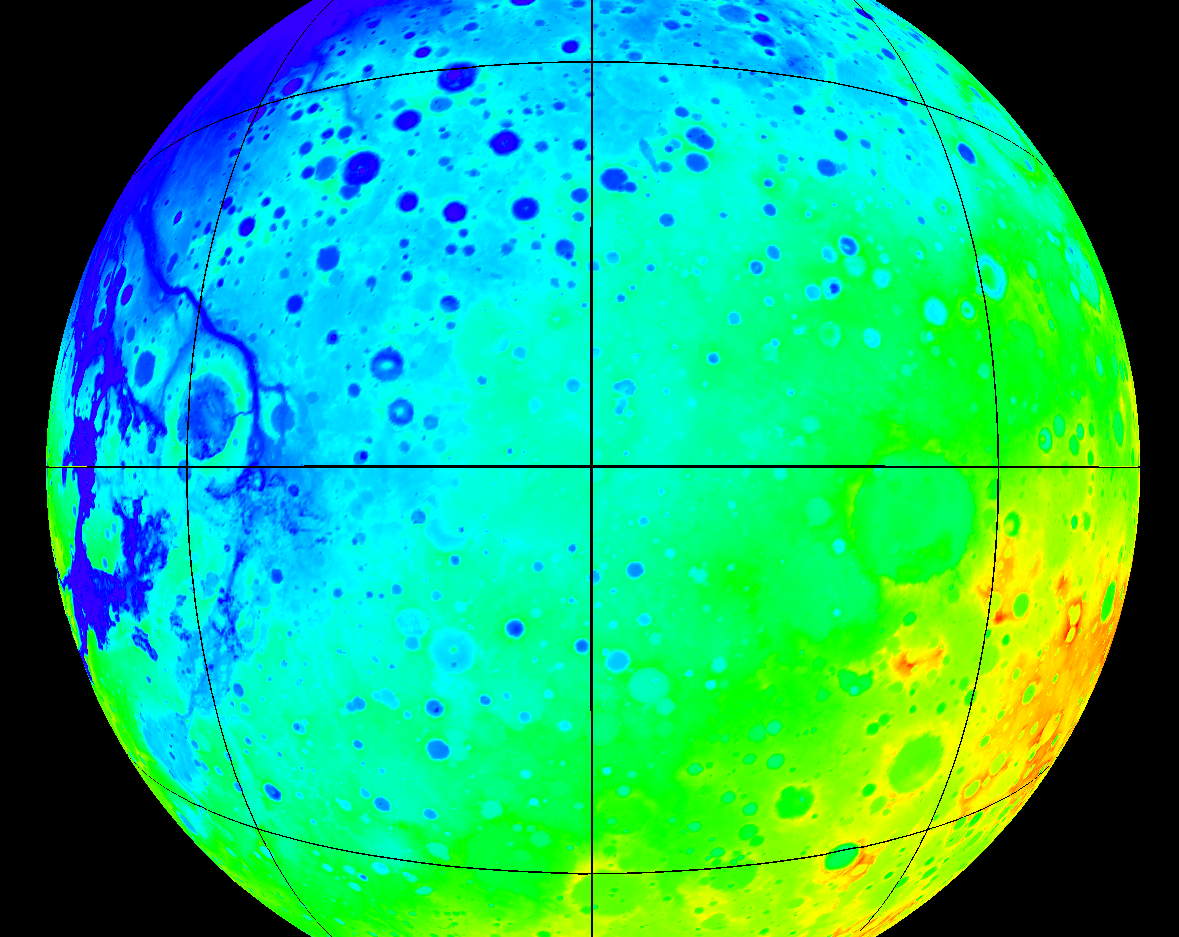
\includegraphics[width=\textwidth]{chunkSeparation.png}
    \subcaption{von Abschnitten}
    \label{chunkSeparation}
  \end{minipage}
  \hfill
  \begin{minipage}[b]{0.45\textwidth}
    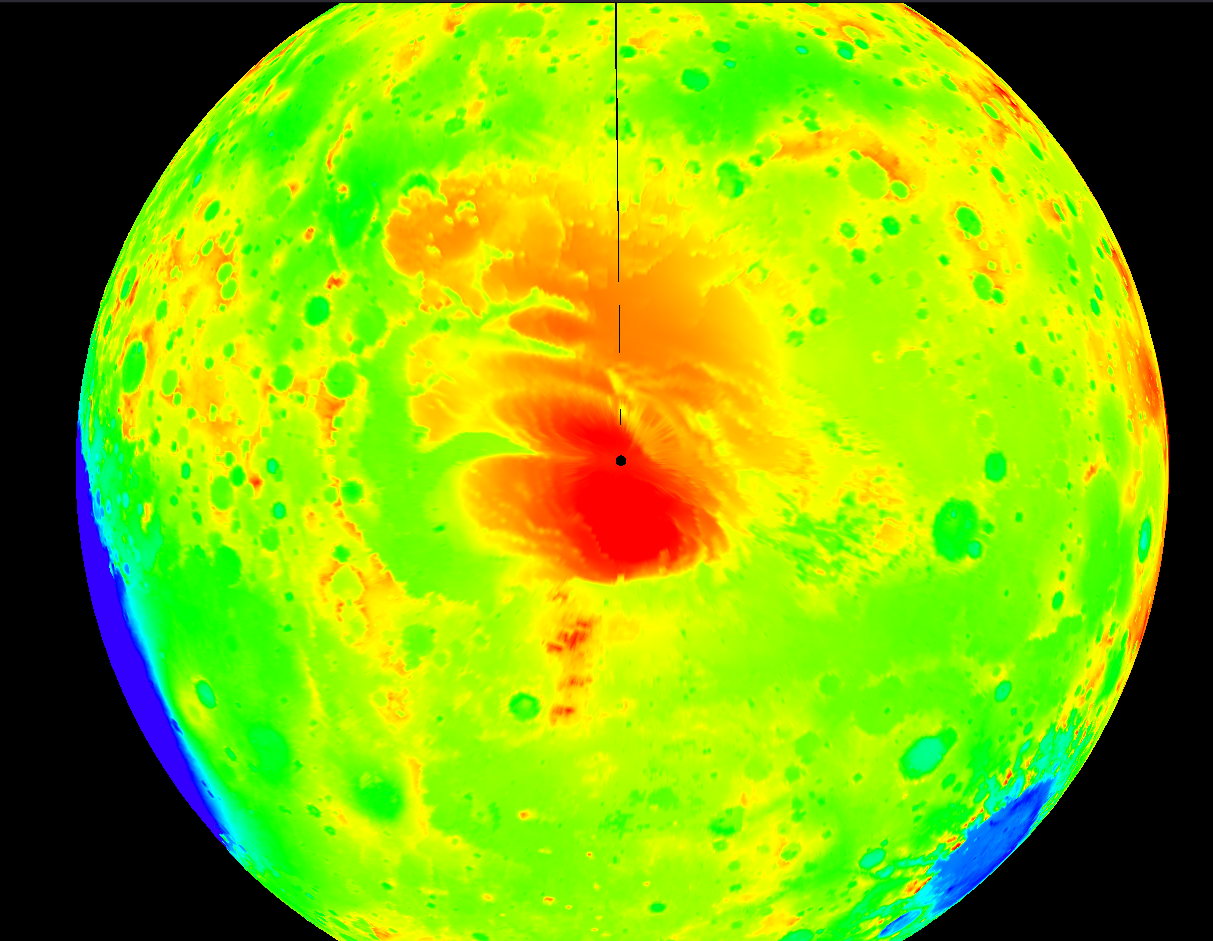
\includegraphics[width=\textwidth]{mapEndSeparation.png}
    \subcaption{des Datensatzes in x- und y-Richtung}
    \label{mapEndSeparation}
  \end{minipage}
  \caption{Abstands-Artefakte an den R\"andern}
\end{figure}

Hier wurde erst überlegt, auf Client Seite die Vertices der Ränder jeweils benachbarter Abschnitte in den eigenen Abschnitt zu kopieren. Da ein Auslesen von Vertexdaten aus dem Grafikspeicher (Vertices sollen möglichst nicht im RAM gehalten werden) jedoch aufwendig ist und die Daten bereits im Backend vorliegen, wurde hier entschieden einfach das Anfrageraster zu vergrößern, sodass sich die Abfragen effektiv überlappen. Ein Problem war dabei, dass die ImageIO-API, welche im Backend genutzt wurde um Ausschnitte aus den Originaldaten auszulesen, nicht zur Lösung des Problems des Verbindens der Ränder des Datensatzes geeignet war. Man musste in x-Richtung effektiv wieder zum Anfang des Datensatzes gesprungen werden, was eine weitere Anfrage und ein mühseliges Kopieren einer weiteren Spalte in eine reihenbasierte Datenstruktur erforderte. In y-Richtung müssen die Werte dagegen die in der Kugelprojektion gegenüberliegenden, aber am selben Rand liegenden Werte, duplizieren, wobei der Versatz jedes x-Wertes durch folgende Formel erlangt werden kann: \[Versatz = (x + Breite / 2) \% Breite\] Die Werte verschieben sich also um die Hälfte der Gesamtbreite, wobei sie beim Überlauf wieder am Anfang starten.

Die Höhenwerte vom Server müssen jetzt in ein indiziertes Polygonnetz überführt werden. Als erstes muss jedem Höhenwert eine Position, also eine x- und z-Koordinate zugewiesen werden. Diese kann aus dem Index i des aktuellen Höhenwertes und dem Reduktionsfaktor r durch die folgende Formel berechnet werden: \[x = (i \% Breite / r) * r\] \[z = floor(i / H\ddot{o}he / r) * r\]
Die bekannten Struktur führt zu einer Bildung einer Gitterstruktur mit einer bekannten Breite und Höhe, die nicht durch den Reduktionsfaktor beeinflusst werden darf. Diese x- und z-Positionen müssen anschließend in Meter umgerechnet werden, wobei jeder Wert einen konstanten, aus der Auflösung berechenbaren Abstand besitzt. Da die Werte in Metern nicht eins zu eins Werten in GL Einheiten entsprechen sollen, werden sie noch entsprechend skaliert. Anschließend muss der Wert in eine Kugelform projiziert werden, wobei hier die einfache Rektangularprojektion, auch Plattkarte genannt, zum Einsatz kommt. Diese ist durch den Datensatz vorgeschrieben, da dieser natürlich ursprünglich aus der echten Kugelform auf eine 2D Form projiziert wurde. Diese Projektion berechnet die Längengrade $\lambda$ und die Breitengrade $\varphi$ an Hand der Positionen x und z, dem Radius R, dem Hauptmeridian $\lambda0$, dem Äquator $\varphi0$, und den Parallelen zum Äquator $\varphi1$ mit folgender Formel: \[\lambda = x / (R * cos(\varphi1)) + \lambda0\] \[\varphi = z / R + \varphi0\]
Sowohl als der Hauptmeridian als auch der Äquator verlaufen erfreulicherweise durch die Mitte des Datensatzes, sodass diese auf $\pi / 2$ bzw. $\pi$ festgesetzt werden können. Die Parallele zum Äquator befindet sich am Äquator, sodass sich die Formel für den Längengrad vereinfacht vereinfacht. Mit Hilfe des Längen- und Breitengrades muss jetzt eine 3D-Koordinate (Kartesisches Koordinatensystem) gefunden werden, wozu die folgende Formel genutzt werden kann: \[x = R * cos(\varphi) * sin(\lambda)\] \[y = -R * sin(\varphi)\] \[z = R * cos(\varphi) * cos(\lambda)\] Hierbei musste die Richtung des Koordinatensystems in OpenGL beachtet werden, was sich von vielen gängigen Ansichten unterschiedet. Wie in Abschnitt \ref{datenmenge} beschrieben hilft die Indexierung dabei, den Datenverbrauch bei der Dopplung von Vertices im Polygonnetz zu verringern. Die Indexierung muss dafür sorgen aus der logischen Gitterstruktur wieder eine eindimensionale Struktur (Reihenfolge der Vertices) zu erstellen. Dabei kann jeder Punkt in der Gitterstruktur, definiert durch x und z, durch die folgende Formel wieder in einen Index umgewandelt werden: \[i = z * width / r + x\]
Für jeden Punkt werden dann zur Bildung eines Rechtecks aus Dreiecken 6 weitere Indizes definiert.

\section{User Interface}
Die fertige User Interface der Anwendung kann in Abbildung \ref{finalUserInterface} betrachtet werden und folgt stark dem geplanten Design. Die einzige relevante Änderung ist der Punkt, dass die Konfiguration der Skala in das Konfigurationspanel verschoben wurde. Dies ist vor allem durch die bessere Unterstützung durch die vom Browser bereitgestellten Inputfelder begründet, welche die Implementierung (z.B. Inputvalidation) stark vereinfachten. Auch wurden die meisten fakultativen Features wie das Koordinatennetz, die Konfigurierbarkeit der Höheneinheiten oder die realistische Beleuchtung durch die Simulation der Sonne aus Zeitgründen nicht implementiert.

\begin{figure}[H]
  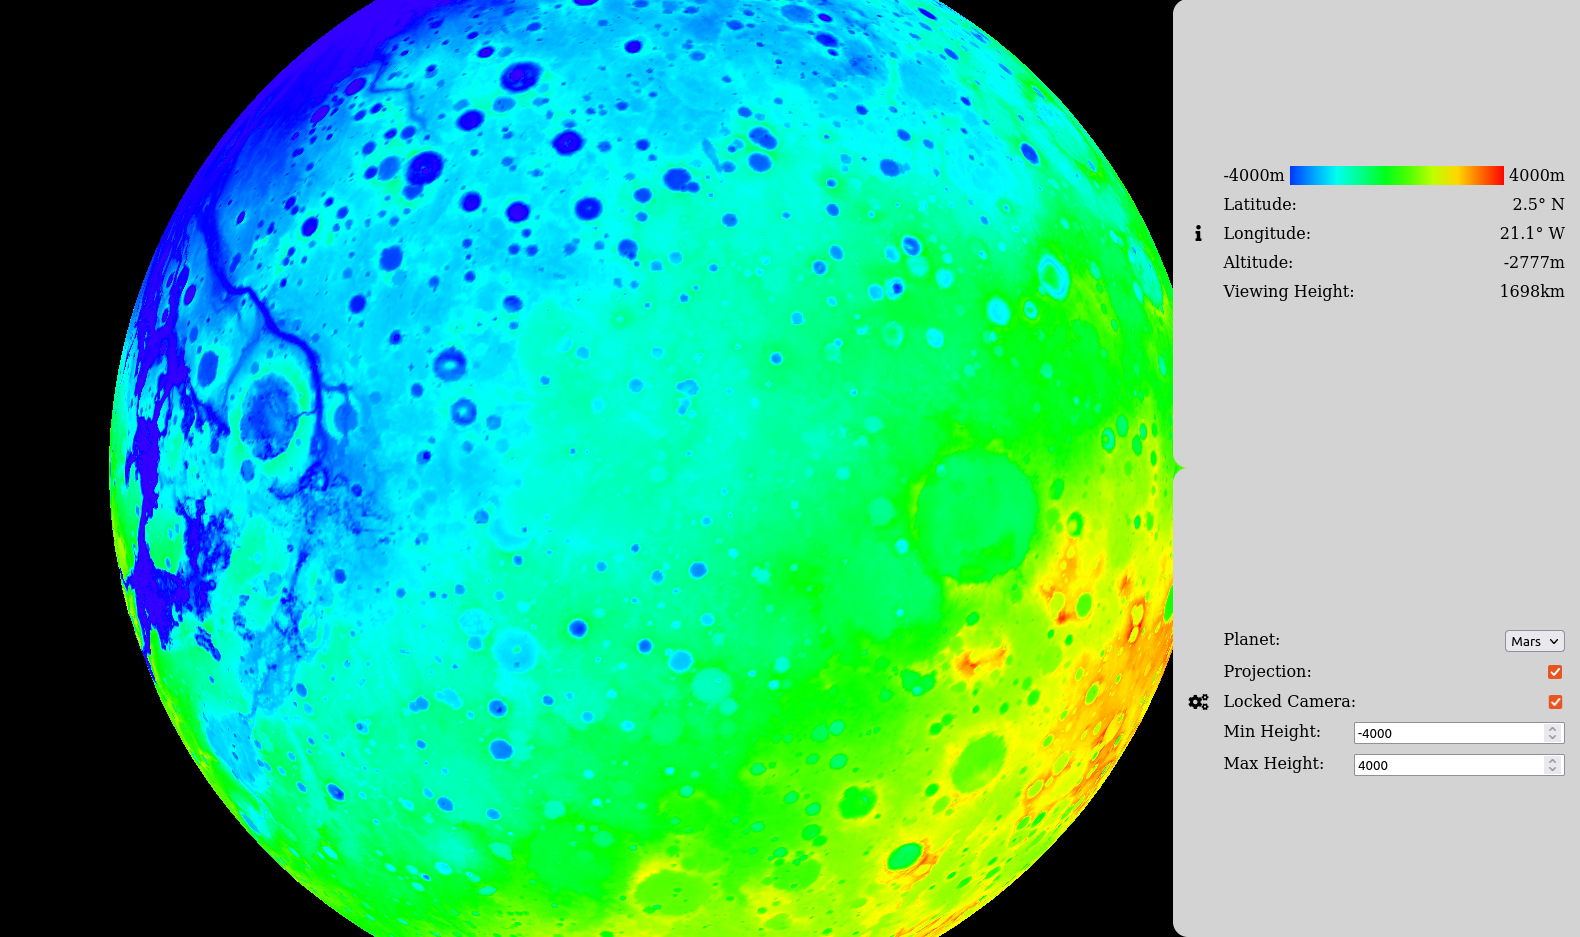
\includegraphics[width=\textwidth,keepaspectratio]{finalUserInterface.png}
  \caption{User Interface der SolarViewer Anwendung}
  \label{finalUserInterface}
\end{figure}

Der grundlegende Ablauf der Anwendung beginnt mit der Initialisierung der Kamera, aller Komponenten und deren Event-Handler und den Shadern. Diese können auf verschiedene Weise eingebunden werden, üblich sind zum Beispiel das Speichern des Shadercodes als String in einer statischen Variable oder als Definition als Inline-Script im HTML. Beide Variationen trennen den Code nicht wirklich vom umliegenden Code, der eine ganz andere Bedeutung hat, und verletzen so das Prinzip des \textit{Separation of concerns}. Stattdessen wurde entschieden, den Shadercode in eigenen Dateien bereitzustellen, welche über den Server ausgeliefert werden. Da der Inhalt externer Scripte aus Sicherheitsgründen allerdings nicht ausgelesen werden können, mussten die Requests manuell ausgeführt werden. Da dies natürlich auch einen Performanceoverhead beinhaltet kann hier nicht von einer optimalen Lösung gesprochen werden. Das eigentliche Rendering läuft in einer Schleife, welche durch die requestAnimationFrame-Funktion auf die Bildwiederholfrequenz begrenzt ist\footnote{ähnlich der vSync Option in nativem Rendering}. Des Weiteren misst die Schleife die vergangene Zeit und sorgt so für Animationen in Kamera und User Interface, die unabhängig von der Performance mit der gleichen Geschwindigkeit ablaufen. 

Die Logik der User Interfaces ist fast ausschließlich in Event-Handlern angesiedelt. Einer davon dient zum Anzeigen der Koordinaten und Höheninformationen beim Mausklick. Dieses Event enthält natürlich nur die Position auf dem Bildschirm, also muss muss als erstes herausgefunden werden, welcher Stelle auf welchem Abschnitt dies entspricht. Auch dafür kommt ein Raycasting zum Einsatz, bei dem alle Abschnitte einzeln überprüft werden müssen. Dieser Punkt im Kartesischen Koordinatensystem muss jetzt mit Hilfe des Radius R wieder in Breiten- und Längengrade umgerechnet werden, wofür die Inverse einer vorigen Funktion zum Einsatz kommt: \[\varphi = asin(-y / R)\] \[\lambda = atan2(x, z)\]
Die atan2 Funktion ist dabei eine spezielle arc tangent Funktion in fast allen Programmiersprachen, welche besondere Spezialfälle bei Parametern bei der Berechnung von $atan(x / z)$ abdeckt und diese auch schneller berechnet. Die Höhe kann wie im Shader berechnet werden, indem der Radius des Planeten vom Punkt auf der Oberfläche abgezogen wird, was im konkreten Fall der Länge des Vertex entspricht. Auch für die Berechnung der Betrachterhöhe kann dieser Trick genutzt werden, wobei hier natürlich die Länge der Kameraposition genutzt werden muss. Auch für die Anzeige der Skala muss die Berechnung der einzelnen Farben mit der gleichen Berechnung wie im Shader durchgeführt werden. Es werden also 10 verschiedene Farben berechnet und dann ein Feld mit linear-gradient Attribut im Frontend gezeigt, welches für ein flüssige Interpolation zwischen den Farben sorgt. Das Konfigurationslogik ist dagegen relativ einfach. Meistens reichen sie die Werte per Uniform direkt an den Shader weiter oder aktivieren die richtige Kameraimplementation, damit diese ihre Events akzeptieren kann. Für das Wechseln der Projektion wird die gesamte Welt neu geladen. Dazu werden als erstes alle Hüllobjekte neu berechnet und dann der Ladeprozess, beschrieben im Abschnitt \ref{dataLoading}, neu ausgeführt. Wichtig ist, dass die stationäre, rotierende Kamera nur bei einem Globus Sinn macht und daher die dynamischere Kamera forciert werden muss. Dabei muss der Konfigurationsparameter allerdings gespeichert werden um ihn beim erneuten Wechsel wieder richtig setzen zu können. Auch ist hier ein wenig Logik bei der Validation der Mindest- und Maximalhöhe vorhanden.

Ein weiterer Punkt ist, dass die Visualisierung immer in der Mitte des Bildschirms sein soll, egal auf welcher Fenstergröße die Visualisierung betrachtet wird. Dazu muss ein resize-Event abgefangen werden, welches beim Ändern der Fenstergröße gefeuert wird. Zum einen muss damit die Projektionsmatrix angepasst werden, sodass Objekte auf dem Bildschirm korrekt in x- und y-Richtung skaliert werden. Zum anderen muss der Viewport an die neuen Dimensionen angepasst werden, sodass die Position auf dem Bildschirm weiterhin stimmt. Außerdem muss die Größe der Canvas angepasst werden, sodass das Layouting des restlichen User Interfaces korrekt ist.

\section{Tests}
Beim Testen der Anwendung hat dieses Projekt das gleiche Probleme aller Grafikprojekte: die Visualisierung kann ohne weiteres nicht automatisch getestet werden. Die Ausgabe auf dem Bildschirm ist zu komplex um daraus Testfälle zu definieren. Auch existieren zu viele Parameter, die das schlussendliche Ergebnis beeinflussen. Und natürlich könnte man Teile des Prozessen testen, zum Beispiel die Erstellung des 3D-Modells auf CPU Seite, allerdings ist es auch dort schwer erwartbare Testfälle zu definieren. Es ist einfach nicht definierbar, wie der Vertex auszusehen hat, der dem n-ten Höhenwert entspricht. Auch die Frage ob Formeln richtig implementiert wurden, lässt sich nur durch die Implementation der Formel im Test testen, was dem Sinn eines Tests widerspricht. Stattdessen wurden in diesem Projekt im Frontend viele manuelle Tests durchgeführt. Zum einen wurde die Visualisierung mit anderen Visualisierungen verglichen. Dabei reichte oft schon ein 2D Bild eines Referenzbildes einer verlässlichen Quelle, im konkreten Fall eine ähnlich eingefärbte Karte des gleichen Datensatzes vom JPL. Außerdem wurde mit Hilfe des Koordinaten und Höhenangaben Features bekannte geographische Features wie den Olympus Mons oder Hellas Planitia gegengeprüft. Da diese Features die Werte an Hand des Vertex berechnen und nicht die originalen Höhenwerte referenzieren, ist es eine recht gute Möglichkeit. Es ist sehr unwahrscheinlich, dass in beiden Implementationen Fehler enthalten sind, die sich gegenseitig aufheben zu richtigen Testresultaten führen. Ansonsten wurde zum Beispiel manuell sichergestellt, dass keine Lücken in der Visualisierung zu sehen sind oder dass die Panels wie geplant aus- und einklappen können. Auch die unterschiedlichen Kamerabewegungen wurden manuell überprüft. Nur bei der Konfiguration der maximalen und minimalen Höhe für die Interpolation wäre ein automatischer Test für das Verhalten bei falschen Benutzereingaben denkbar gewesen. 

Im Backend dagegen wurde jede öffentliche Methode zumindest mit einem Testfall abgedeckt. Relativ viel Aufwand wurde beim Testen der Redundanzentfernung betrieben. Hier wurde ein unbekannter Algorithmus getestet, der insbesondere keine optimale Lösung finden kann. Dadurch wurden viele Testfälle definiert, die prüfen, ob sehr einfache Optimierungsfälle, wie zum Beispiel die Überprüfung aller Alternativen bei nachfolgenden linearen Abhängigkeiten, eingehalten wurden. Auch Edge Cases konnten hier schön abgedeckt werden, zum Beispiel Fälle von Redundanzen die am Rand eines Abschnitts liegen oder bei denen redundante Teilraster nebeneinander liegen. Für den Endpoint wurden Tests geschrieben, die sicherstellen, dass die Redundanzentfernung korrekt ausgeführt wird und das alle Parameter (Position, Dimension, Reduktionsfaktor) korrekt behandelt werden.
